%%% Local Variables:
%%% mode: latex
%%% TeX-master: "learning_with_kernels"
%%% End:


\tikzset{
  noise_pt/.style={solidity,fill=black,draw},  
  pos_pt/.style={circle,minimum width=.4ex, fill=none,draw},
  neg_pt/.style={circle,minimum width=.4ex, fill=black,thick,draw},
  pos_sv/.style={solid,circle,minimum width=.6ex, fill=black,thick,draw=white},
  neg_sv/.style={solid,circle,minimum width=.6ex, fill=none,thick,draw},
}
  
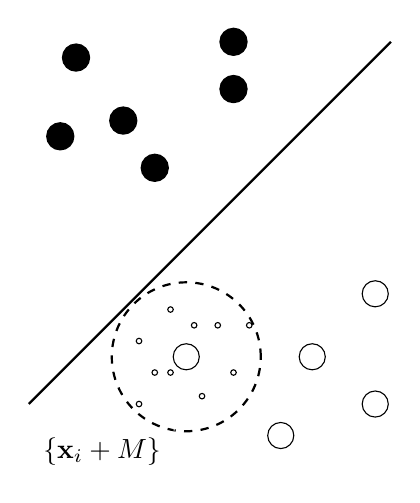
\begin{tikzpicture}[
  scale=2,
  every node/.style={color=black},
  important line/.style={thick},
  dashed line/.style={dashed, thin},
  ]

  \draw[important line]
       (.7,.7) coordinate (lines) -- (3,3) coordinate (linee);

   \foreach \Point in {(1.5,2.2), (.9,2.4), (1.3,2.5), (2,3), (1,2.9), (2,2.7)}{
     \draw \Point node[neg_pt]{};
   }

   \foreach \Point in {(1.7, 1), (2.9,1.4), (2.3,.5), (2.9,.7), (2.5,1)}{
     \draw \Point node[pos_pt]{};
   }

   \draw node[circle,minimum width=12.5ex,fill=none,thick,draw,dashed] at (1.7, 1) {};

   \foreach \Point in {(1.4,1.1),(1.6,.9),(2.0,.9),(1.4,0.7),(1.8,0.75),(1.9,1.2),(2.1,1.2),(1.75,1.2),(1.5, 0.9),(1.6,1.3)} {
     \draw \Point circle[radius=.5pt];
   }

   \draw[dashed, thin,white] (1.7, 1) -- (1.6,0.4)
   node[above, left] {$\{ \mathbf{x}_i + M \}$};
   
 \end{tikzpicture}
